\documentclass{frontiersSCNS}
\usepackage{url,hyperref,lineno,microtype,subcaption}
\usepackage[onehalfspacing]{setspace}
\usepackage{float}


\linenumbers

\usepackage[utf8]{inputenc}
\floatplacement{figure}{H}

\def\keyFont{\fontsize{8}{11}\helveticabold }
\def\firstAuthorLast{Villaseñor-Derbez {et~al.}}
\def\Authors{Juan Carlos Villaseñor-Derbez\(^{1,2,*}\), Eréndira
Aceves-Bueno\(^{1}\), Álvin Suarez\(^{2}\), Stuart Fulton\(^{2}\),
Arturo Hernández-Velasco\(^{2}\), Jorge Torre\(^{2}\), Fiorenza
Micheli\(^{3}\)}
% Affiliations should be keyed to the author's name with superscript numbers and be listed as follows: Laboratory, Institute, Department, Organization, City, State abbreviation (USA, Canada, Australia), and Country (without detailed address information such as city zip codes or street names).
% If one of the authors has a change of address, list the new address below the correspondence details using a superscript symbol and use the same symbol to indicate the author in the author list.
\def\Address{\(^{1}\)Bren School of Environmental Science and Management, University
of California, Santa Barbara, Santa Barbara, CA,
USA\newline \(^{2}\)Comunidad y Biodiversidad A.C., Guaymas, Sonora,
Mexico\newline \(^{3}\)Hopkins Marine Station and Center for Ocean
Solutions, Stanford University, Pacific Grove, CA, USA}
% The Corresponding Author should be marked with an asterisk
% Provide the exact contact address (this time including street name and city zip code) and email of the corresponding author
\def\corrAuthor{Juan Carlos Villaseñor-Derbez, Bren Hall, University of California,
Santa Barbara, Santa Barbara, CA, 93106}

\def\corrEmail{\href{mailto:juancarlos@ucsb.edu}{\nolinkurl{juancarlos@ucsb.edu}}}

\usepackage{amsthm}
\newtheorem{theorem}{Theorem}[section]
\newtheorem{lemma}{Lemma}[section]
\theoremstyle{definition}
\newtheorem{definition}{Definition}[section]
\newtheorem{corollary}{Corollary}[section]
\newtheorem{proposition}{Proposition}[section]
\theoremstyle{definition}
\newtheorem{example}{Example}[section]
\theoremstyle{definition}
\newtheorem{exercise}{Exercise}[section]
\theoremstyle{remark}
\newtheorem*{remark}{Remark}
\newtheorem*{solution}{Solution}
\begin{document}
\onecolumn
\firstpage{1}

\title[Community-based marine reserves]{Effectiveness of community-based marine reserves in small-scale
fisheries} 

\author[\firstAuthorLast ]{\Authors} %This field will be automatically populated
\address{} %This field will be automatically populated
\correspondance{} %This field will be automatically populated

\extraAuth{}

\maketitle



\begin{abstract}

Coastal marine ecosystems provide livelihoods for small-scale fishers
and coastal communities around the world. Artisanal fisheries face great
challenges since they are difficult to monitor, enforce, and manage.
Combining territorial user rights for fisheries (TURF) with no-take
marine reserves to create TURF-reserves is believed to improve the
performance of small-scale fisheries by buffering fisheries from
environmental variability and management errors, while ensuring that
fishers reap the benefits of conservation investments. In the last six
years, and following a 2012 regulation, 18 TURF-reserves have been
implemented in Mexico; their effectiveness has not been formally
evaluated. We combine causal inference techniques and a
social-ecological systems framework to provide a holistic evaluation of
community-based TURF reserves in three coastal communities in Mexico. We
find that while reserves have not yet achieved their stated goal of
increasing lobster densities, they continue to receive significant
support from the fishing communities. A lack of ecological and
socioeconomic effects likely results from a combination of factors.
First, the lobster fisheries are already well managed, and it is
unlikely that reserves might have a detectable effect. Second, some of
the reserves are not large enough to protect lobsters' home ranges.
Third, some of these reserves might be too young for the effects to
show. However, these reserves have shaped small-scale fishers' way of
thinking about marine conservation, which can provide a foundation for
establishing additional, larger marine reserves needed to effectively
conserve mobile species.




\medskip
\tiny
 \keyFont{ \section{Keywords:} TURF-reserves, Causal Inference, Social-Ecological Systems, Marine
Protected Areas, Marine Conservation, Small-Scale Fisheries}



\end{abstract}


\clearpage

\section{Introduction}\label{introduction}

Marine ecosystems around the world sustain significant impacts due to
overfishing and unsustainable fishing practices
\citep{halpern_2008-dK,worm_2006-IB,pauly_2005-qV}. In particular,
artisanal fisheries face great challenges since they tend to be hard to
monitor and enforce \citep{costello_2012}. Recent research shows that
combining Territorial Use Rights for Fisheries (TURFs) with no-take
marine reserves (MR) can greatly improve the performance of coastal
fisheries and the health of the local resouces
\citep{costello_2010-Ix,lester_2017}. Commonly known as TURF-Reserves,
these systems increase the benefits of spatial access rights allowing
the maintainance of healthy resources
\citep{afflerbach_2014-HP,lester_2017}. Although in theory these systems
are successful \citep{costello_2010-Ix}, there is little empirical
evidence of their effectiveness and the drivers of their success
\citep{afflerbach_2014-HP,lester_2017,smallhornwest_2018}.

The performance of these systems depends on how environmental and social
factors combine and interact. The science of marine reserves has largely
focused on understanding the ecological effects of these areas, which
include increased biomass, species richness, and densities of organisms
within the protected regions, climate change mitigation, and protection
from environmental variability
\citep{lester_2009-Ks,giakoumi_2017-V2,sala_2017-69,roberts_2017-J9,micheli_2012-EU}.
Modelling studies show that fishery benefits of marine reserves depend
on initial stock status and the management under which the fishery
operates, as well as reserve size and the amount of larvae exported from
these \citep{hilborn_2006,krueck_2017-J1,deleo_2015}. Other research has
focused on the relationship between socioeconomic and governance
structures and reserve effectiveness
\citep{halpern_2013,lpezangarita_2014,mascia_2017-m_}. However, to our
knowledge, no studies exist that evaluate TURF-reserves from both a
social and ecological perspective. This is especially important in
social-ecological coastal systems dominated by close interaction and
feedbacks between people and natural resources \citep{ostrom_2009-hg}.

TURF-reserves can be created as community-based marine reserves,
voluntarily established and enforced by local communities. This
bottom-up approach increases compliance and self-enforcement
\citep{gelcich_2015-Gw,espinosaromero_2014-PY,beger_2004-Y8}.
Community-based spatial closures occur in different contexts, like the
\emph{kapu} or \emph{ra'ui} areas in the Pacific Islands
\citep{bohnsack_2004,johannes_2002}. However, without legal recognition
no-take regulations are difficult to enforce and fishers rely on the
exclusive access granted by the TURF. In an effort to bridge this
normative gap, Civil Society Organizations (CSOs) have served as a link
between fishers and government, and set out to create a legal framework
that solve this governance issue. In Mexico, a new norm was created in
2014 allowing fishers to request the legal recognition of
community-based reserves as ``Fish Refuge'' (\emph{Zona de Refugio
Pesquero}; \citet{nom}). Fish refuges can be implemented as temporal or
partial reserves, which can protect one, some, or all resources within
their boundaries. Since 2012, 45 of Fish Refuges have been created along
the Pacific, Gulf of California, and Mexican Caribbean coastlines, with
18 of them implemented as TURF-reserves. However, their effectiveness
has not yet been formally evaluated and reported in the scientific
literature.

Here, we combine causal inference techniques and a social-ecological
systems framework to provide a holistic evaluation of community-based
marine reserves in three coastal communities in Mexico. These three case
studies span a range of ecological and social conditions representative
of different regions of Mexico. The objective of this work is twofold.
First, to provide a triple bottom line evaluation of the effectiveness
of community-based marine reserves that can inform similar processes in
other countries. Second, to evaluate the effectiveness of TURF-reserves
established as Fish Refuges in Mexico to identify opportunities where
improvement or adjustment might lead to increased effectiveness. We draw
from lessons learned in these three case studies and provide management
recommendations to maximize the effectiveness of community-based marine
reserves in small-scale fisheries in Mexico and in other regions around
the world that are using this tool to manage and rebuild their coastal
fisheries.

\section{Methods}\label{methods}

\subsection{Study area}\label{study-area}

We evaluate three TURF-reserves in Mexico (Fig \ref{fig:map}A). The
first one was created by the \emph{Buzos y Pescadores de la Baja
California} fishing cooperative, located in Isla Natividad in the Baja
California Peninsula (Fig \ref{fig:map}B). The main fishery in the
island is the spiny lobster (\emph{Panulirus interruptus}), but other
resources like finfish, sea cucumber, read sea urchin, snail, and
abalone are also an important source of income. In 2006, the community
decided to implement two marine reserves within their fishing grounds to
protect commercially important invertebrate species; mainly lobster and
abalone. While these reserves obtained legal recognition only in 2018,
they have been well enforced since their implementation.

The other two TURF-reserves are located in Maria Elena and Punta
Herrero, in the Yucatan Peninsula (Fig \ref{fig:map}C). In contrast with
Isla Nativdad, which hosts a well established fishing community, Maria
Elena is a fishing camp --visited intermittently during the fishing
season-- belonging to the Cozumel fishing cooperative (\emph{SCPP
Cozumel}); Punta Herrero is home to the \emph{SCPP José María Azcorra}
cooperative, and similar to Isla Natividad hosts a local community.
Their main fishery is the Caribbean spiny lobster (\emph{Panulirus
argus}), but they also target finfish in the off-season. Maria Elena and
Punta Herrero established eight marine reserves in 2012, and four marine
reserves in 2013, respectively. All these reserves have been legally
recognized as Fishing Refuges since their creation
\citep{dof_website_2012,dof_website_2013}.

These communities are representative of their region in terms of
ecology, socioeconomic, and governance aspects. Isla Natividad, for
example, is part of a greater group of fishing cooperatives belonging to
a Federation of Fishing Cooperatives. This group has been identified as
a cohesive group that often cooperates to better manage their resources
\citep{mccay_2017-1m,mccay_2014-CN,acevesbueno_2017}. Likewise, Maria
Elena and Punta Herrero are representative of fishing cooperatives in
the Mexican Caribbean, which are also part of a regional Federation.
Together, these three communities provide an accurate representation of
other fishing communities in each of their regions. While each region
has additional communities that have established community-based
TURF-reserves, available data would not allow us to perform the in-depth
analysis that we undertake. Yet, given the similarities among
communities and the socioeconomic and governance setting under which
they opperate, it is safe to cautiously generalize our results to other
communities in Mexico and other regions around the world.

\subsection{Data collection}\label{data-collection}

We use three main sources of information to evaluate these reserves
across the ecological, socioeconomic, and governance dimensions.
Ecological data come from the annual ecological monitoring of reserve
and control areas, carried out by members from each community and
personnel from the Mexican CSO \emph{Comunidad y Biodiversidad}
(\href{www.cobi.org.mx}{COBI}). Trained divers record richness and
abundances of fish and invertebrate species along replicate transects
(30x 2 m each) at depths 5-20 m in the reserves and control sites
\citep{fulton_2018,fulton_2019}. Size structures are also collected
during fish surveys. We define control sites as regions with habitat
characteristics similar to the corresponding reserves, and that
presumably had a similar probability of being selected as reserves
during the design phase. We focus our evaluation on sites where data are
available for reserve and control sites, before and after the
implementation of the reserve. This provides us with a
Before-After-Control-Impact (\emph{i.e.} BACI) sampling design that
allows us to capture and control for temporal and spatial dynamics
\citep{depalma_2018,ferraro_2006-oW}. BACI designs and causal inference
techniques have proven effective to evaluate marine reserves, as they
allow us to causally attribute observed changes to the intervention
\citep{moland_2013-VP,Villasenor-Derbez_2018}. All sites were surveyed
annually, and at least once before implementation of the reserves.

Socioeconomic data come from landing receipts reported to the National
Commission for Aquaculture and Fisheries (\emph{Comisión Nacional de
Acuacultura y Pesca}; CONAPESCA). Data contain monthly lobster landings
(Kg) and revenues (MXP) for cooperatives with and without marine
reserves. Cooperatives incorporated in this analysis belong to larger
regional-level Cooperative Federations, and are exposed to the same
markets and institutional frameworks, making them plausible controls
\citep{mccay_2017-1m,ayer_2018}. Landings and revenues were aggregated
at the cooperative-year level, and revenues were adjusted to represent
2014 values by the Consumer Price Index for Mexico \citep{oecd_2017-VV}
as:

\begin{equation}
I_t = RI_t\times\frac{CPI_t}{CPI_T}
\label{eqn:cpi}
\end{equation}

Where \(I_t\) represents the adjusted income for year \(t\) as the
product between the reported income for that year and the ratio between
the consumer price index in that year (\(CPI_t\)) to the most recent
year's consumer price index (\(CPI_T\)).

Data for the operationalization of the social-ecological system were
collected at the community--level from official documents used in the
creation and designation of the marine reserves
\citep{dof_website_2012,dof_website_2013,dof_website_2018} and based on
the authors' experience and knowledge of the communities. These include
information on the resource system, the resource units, actors, and the
governance system itself (Table \ref{table:ses}).

\subsection{Data analysis}\label{data-analysis}

We evaluate the effect that marine reserves have had on four ecological
and two socioeconomic indicators (Table \ref{table:indicators}). Recall
that reserves were implemented to protect lobster and other benthic
invertebrates. However, we also use the available fish data to test for
associated co-benefits.

We use a difference-in-differences analysis to evaluate these
indicators. This approach allows us to estimate the effect that the
reserve had by comparing trends across time and treatments
\citep{moland_2013-VP,Villasenor-Derbez_2018}. The analysis of
ecological indicators is performed with a multiple linear regression of
the form:

\begin{equation}
I_{itj} = \alpha + \gamma_{t} Year_t + \beta Zone_i + \lambda_{t} Year_t\times Zone_i + \sigma_jSpp_j + \epsilon
\label{eqn:reg_bio}
\end{equation}

Where year-fixed effects are represented by \(\gamma_{it} Year_t\), and
\(\beta Zone_i\) captures the difference between reserve (\(Zone = 1\))
and control (\(Zone = 0\)) sites. The interaction term
\(\lambda_{it} Year_t\times Zone_i\) represents the mean change in the
indicator inside the reserve, for year \(t\), with respect to the year
of implementation in the control site. When evaluating biomass and
densities of the invertebrate or fish communities, we include
\(\sigma_j\) to control for species-fixed effects.

Socioeconomic indicators are evaluated with a similar approach. Due to
data constrains, we only evaluate socioeconomic data for Isla Natividad
(2000 - 2014) and Maria Elena (2006 - 2013). Neighboring communities are
used as counterfactuals that allow us to control for unobserved
time-invariants. Each focal community (Isla Natividad and Maria Elena)
has three counterfactual communities.

\begin{equation}
I = \alpha + \gamma_{t} Year_t + \beta Treated_i + \lambda_{t} Year_t\times Treated_i + \sigma_jCom_j +\epsilon
\label{eqn:soc_reg}
\end{equation}

The model interpretation remains as for Eq \ref{eqn:reg_bio}, but in
this case the \(Treated\) dummy variable indicates if the community has
a reserve (\(Treated = 1\)) or not (\(Treated = 0\)) and \(\sigma_jCom\)
captures community-level fixed-effects. These regression models allow us
to establish a causal link between the implementation of marine reserves
and the observed trends by accounting for temporal and spatial dynamics
\citep{depalma_2018}. The effect of the reserve is captured by the
\(\lambda_t\) coefficient, and represents the difference observed
between the control site before the implementation of the reserve and
the treated sites at time \(t\) after controlling for other time and
space variations (\emph{i.e.} \(\gamma_t\) and \(\beta\) respectively).
All model coefficients were estimated via ordinary least-squares and
heteroskedastic-robust standard errors \citep{zeileis_2004-7n}. All
analyses were performed in R 3.5.0 and R Studio 1.1.453 \citep{R_2018}.
Data and code are available on
\href{https://github.com/jcvdav/ReserveEffect}{github.com}.

We use the social-ecologycal system (SES) framework to evaluate each
community as a means of providing an explanation to the biological and
socioeconomic results. The use the SES framework standardizes our
analysis and allows us to communicate our results in a common language
across fields. We based our variable selection primarily on
\citet{leslie_2015-na,basurto_2013-oq}, who have previously analyzed
Mexican fishing cooperatives using this framework. We also incorporate
other relevant information following \citet{difranco_2016-Xw} and
\citet{edgar_2014-UO}. Table \ref{table:ses} shows the selected
variables, their definition and selected indicators.

\section{Results}\label{results}

The following sections present the effect that marine reserves had on
each of the biological and socioeconomic indicators for each coastal
community. Results are presented in terms of the difference through time
and across sites, relative to the control site on the year of
implementation (\emph{i.e.} effect size \(\lambda_t\)). We also provide
an overview of the governance settings of each community, and discuss
how these might be related to the effectiveness and performance of the
reserves.

\subsection{Biological effects}\label{biological-effects}

Indicators showed ambiguous responses through time for each reserve.
Figure \ref{fig:indicators}A shows positive effect sizes for lobster
densities in Isla Natividad and Punta Herrero during the first years,
but the effect is eroded through time. In the case of Maria Elena,
positive changes were observed in the third and forth year. These
effects are in the order of 0.2 extra organisms \(\mathrm{m}^{-2}\) for
Isla Natividad and Punta Herrero, and 0.01 organisms \(\mathrm{m}^{-2}\)
for Maria Elena, but are not significantly different from zero
(\(p > 0.05\)). Likewise, no changes were detected in fish biomass or
invertebrate and fish densities (\ref{fig:indicators}B-D), where effect
sizes oscillated around zero without clear trends. Full tables with
model coefficients are presented in the supplementary materials (S1
Table, S2 Table, S3 Table).

\subsection{Socioeconomic effects}\label{socioeconomic-effects}

Lobster landings and revenue were only available for Isla Natividad and
Maria Elena (Fig \ref{fig:lobsters}). For all years before
implementation, the effect sizes are close to zero, indicating that the
control and treatment sites have similar pre-treatment trends,
suggesting that these are plausible controls. However, effect sizes do
not change after the implementation of the reserve. Interestingly, the
negative effect observed for Isla Natividad on year 5 correspond to the
2011 hypoxia events. The only positive change observed in lobster
landings is for Isla Natividad in 2014 (\(p < 0.1\)). The three years of
post-implementation data for Maria Elena do not show a significant
effect of the reserve. Isla Natividad shows higher revenues after the
implementation of the reserve, as compared to the control communities.
However, these changes are not significant and are associated to
increased variation. Full tables with model coefficients are presented
in the supplementary materials (S4 Table, S5 Table).

\subsection{Governance}\label{governance}

Our analysis of the SES (Table \ref{table:ses}) shows that all analyzed
communities share similarities known to foster sustainable resource
management and increase reserve effectiveness. For example, fishers
opperate within clearly outlined TURFs (RS2, GS6.1.4.3) that provide
exclusive access to resources and reserves. Along with their relatively
small groups (A1 - Number of relevant actors), Isolation (A3),
Operational rules (GS6.2), Social monitoring (GS9.1), and Graduated
sanctions (GS10.1), these fisheries have solid governance structures
that enable them to monitor their resources and enforce rules to ensure
sustainable management. In general, success of conservation initiatives
depends on the incentives of local communities to maintain a healthy
status of the resources upon which they depend \citep{jupiter_2017}. Due
to the clarity of access rights and isolation, the benefits of
conservation directly benefit the members of the fishing cooperatives,
which have favored the development of efficient community-based
enforcement systems. However, our SES analysis also highlights factors
that might hinder reserve performance or mask outcomes While total
reserve size ranges from 0.2\% to 3.7\% of the TURF area, individual
reserves are often small (RS3), and relatively young (RS5).
Additionally, fishers harvest healthy stocks (RS4.1), and it's unlikely
that marine reserves will result in increased catches.

\section{Discussion}\label{discussion}

Our results indicate that these TURF-reserves have not increased lobster
densities. Additionally, no co-benefits were identified when using other
ecological indicators other than the previously reported buffering
effect that reserves can have to environmental variability in Isla
Natividad \citep{micheli_2012-EU}. The socioeconomic indicators
pertaining landings and revenues showed little to no change after
reserve implementation. The coastal ecosystems where these reserves are
located have been profoundly affected by climatic and oceanographic
extremes, including warming events, extreme storms and prolonged hypoxia
\citep{micheli_2012-EU,woodson}. Despite the lack of evidence of the
effectiveness of these reserves, most of the communities show a positive
perception about their performance and continue to support their
presence \citep{ayer_2018}. Understanding the social-ecological context
in which these communities and their reserves operate might provide
insights to this.

Some works evaluate marine reserves by performing inside-outside
\citep{guidetti_2014-8Z,friedlander_2017-oI,rodriguez_2017-PD} or
before-after comparisons \citep{betti_2017-lq}. The first approach does
not address temporal variability, and the second can not distinguish
between the temporal trends in a reserve and the entire system
\citep{depalma_2018}. Our approach to evaluate the temporal and spatial
changes provides a more robust measure of reserve effectiveness. For
example, we capture previously described patterns like the rapid
increase observed for lobster densities in Isla Natividad on the sixth
year (\emph{i.e.} 2012; Fig. \ref{fig:indicators}A) -a year after the
hypoxia events described by \citet{micheli_2012-EU}- which caused mass
mortality of sedentary organisms such as abalone and sea urchins, but
not lobster and finfish. Yet, our empirical approach assumes control
sites are a plausible counterfactual for treated sites. This implies
that treated sites would have followed the same trend as control sites,
had the reserves not been implemented. Nonetheless, temporal trends for
each site don't show any significant increases (S1 Table, S2 Table, S3
Table), supporting our findings of lack of change in the indicators
used.

A first possible explanation for the lack of effectivenes may be the
young age of the reserves. Literature shows that age and enforcement are
important factors that influence reserve effectiveness
\citep{edgar_2014-UO,babcock_2010}. Isla Natividad has the oldest
reserves, and our SES analysis suggests that all communities have a
well-established community-based enforcement system. With these
characteristics, one would expect the reserves to be effective. Maria
Elena and Punta Herrero are relatively young reserves (\emph{i.e.}
\textless{} 6 years old) and effects may not yet be evident due to the
short duration of protection, relative to the life histories of the
protected species; other community-based marine reserves in tropical
ecosystems may take up to six years to show a spillover effect
\citep{dasilva_2015-zX}.

Another key condition for effectiveness is reserve size
\citep{edgar_2014-UO}, and the lack of effectiveness can perhaps be
attributed to poor ecological coherence in reserve design (\emph{sensu}
\citet{rees_2018}. Previous research has shown that reserves in Isla
Natividad yield fishery benefits for the abalone fishery
\citep{rossetto_2015-V0}. Abalone are less mobile than lobsters, and
perhaps the reserves provide enough protection to these sedentary
invertebrates, but not lobsters. Design principles developed by
\citet{green_2017} for marine reserves in the Caribbean state that
reserves ``should be more than twice the size of the home range of
adults and juveniles'', and suggest that reserves seeking to protect
spiny lobsters should have at least 14 km across. Furthermore, fishers
may favor implementation of reserves that pose low fishing costs due to
their small size or location. Our analysis of economic data supports
this, as neither landings nor revenues showed the expected short-term
costs associated to the first years of reserve implementation
\citep{ovando_2016-Wg}.

Even if reserves had appropriate sizes and were placed in optimal
locations, there are other plausible explanations for the observed
patterns. For instance, marine reserves are only likely to provide
fisheries benefits if initial population sizes are low and the fishery
is poorly managed \citep{hilborn_2006}. Both lobster fisheries were
certified by the Marine Stewardship Council \citep{prezramrez_2016-J1}.
Additionally, lobster fisheries are managed via species-specific minimum
catch sizes, seasonal closures, protection of ``berried'' females, and
escapement windows where traps are allowed \citep{dof_website_1993}. It
is uncertain whether such a well-managed fishery will experience
additional benefits from marine reserves. Additionally,
\citet{gelcich_2008} have shown that TURFs alone can have greater
biomass and richness than areas operating under open acces. These
increased attributes perhaps minimize the difference between TURF and
reserve, making it difficult to detect such a small difference. Further
research should focus on evaluating sites in the reserve, TURF, and open
access areas or similar Fish Refuges established without the presence of
TURFs where the impact of ther eserves might be larger.

While the evaluated reserves have failed to provide fishery benefits up
to now, there are a number of additional ecological, fisheries, and
social benefits. Marine reserves provide protection to a wider range of
species and vulnerable habitat, like coral reefs. These sites can serve
as an insurance against uncertainty and errors in fisheries management,
as well as environmental shocks
\citep{hilborn_2004,hilborn_2006,micheli_2012-EU,aalto}. Self-regulation
of fishing effort (\emph{i.e.} reduction in harvest) can serve as a way
to compensate for future declines associated to environmental variation
\citep{finkbeiner_2018}. Embarking in a marine conservation project can
bring the community together, which promotes social cohesion and builds
social capital \citep{fulton_2019}. Showing commitment to marine
conservation and sustainable fishing practices allows fishers to have
greater bargaining power and leverage over fisheries management
\citep{prezramrez_2012}. Furthermore, the lack of effectiveness observed
in these reserves may not be generalizable to other reserves established
under the same legal frameowrk (\emph{i.e.} Fish Refges) in Mexico, and
future research should aim at evaluating other areas that have also been
established as bottom-up processes bt without the presence of TURFs
(\emph{e.g.} \citet{dof_websiteC_2012}), or others established through a
top-down process (\emph{i.e.} \citet{dof_websiteU_2018}).

Previous studies have evaluated the potential of implementing marine
reserves in Baja California and connect them to the existing network in
California \citep{arafehdalmau_2017}. Community-based marine reserves in
small-scale fisheries can be helpful conservation and fishery management
tools when appropriately implemented. Lessons learned from these cases
can guide implementation of community-based marine reserves elsewhere.
For the particular case of the marine reserves that we evaluate, the
possibility of expanding reserves or merging existing polygons into
larger areas should be evaluated and proposed to the communities. At the
broader scale, having full community support surely represents an
advantage, but it is important that marine reserves meet essential
design principles such as size and placement. Community-based marine
reserves might have more benefits that result from indirect effects of
the reserves, which should be taken into account when evaluating the
outcomes of similar projects.

\section*{Conflict of Interest Statement}

The authors declare that the research was conducted in the absence of
any commercial or financial relationships that could be construed as a
potential conflict of interest.

\section*{Author Contributions}

JC and EA analyzed and interpreted data, discussed the results, and
wrote the first draft. AHV coordinated fieldwork and collected the data.
AS, AHV, SF, JT, and FM discussed the results and edited the manuscript.

\section*{Funding}

JCVD recevied funding from CONACyT (Beca de Posgrados en el extranjero,
CVU 669403) and the Latin American Fisheries Fellowship Program. AS,
AHV, SF and JT received funding from Marisla Foundation, Packard
Foundation, Walton Family Foundation, Summit Foundation, and Oak
Foundation.

\section*{Acknowledgments}

The authors wish to acknowledge Imelda Amador for contributions on the
governance data, as well as pre-processing biological data. This study
would have not been possible without the effort by members of the
fishing communities here mentioned, who participated in the
data-collection process.

\clearpage

\bibliographystyle{frontiersinSCNS_ENG_HUMS}\bibliography{references}

\clearpage

\section*{Figure captions}

\begin{figure}
\centering
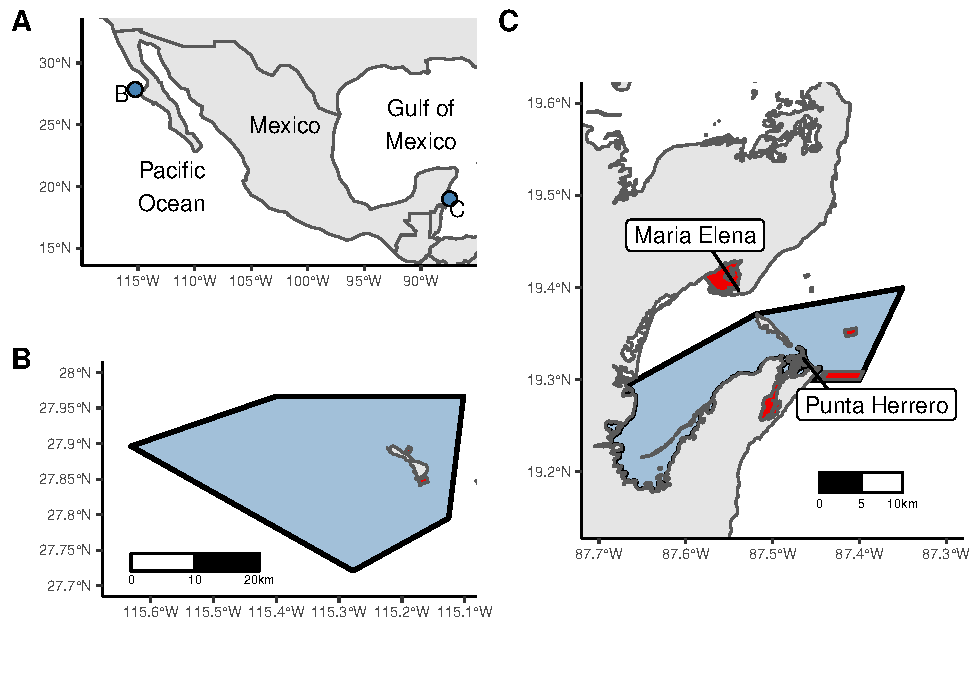
\includegraphics{Villasenor-Derbez_files/figure-latex/unnamed-chunk-7-1.pdf}
\caption{\label{fig:unnamed-chunk-7}\label{fig:map}Location of the three
coastal communities studied (A). Isla Natividad (B) is located off the
Baja California Peninsula, Maria Elena and Punta Herrero (C) are located
in the Yucatan Peninsula. Blue polygons represent the TURFs, and red
polygons the marine reserves.}
\end{figure}

\begin{figure}
\centering
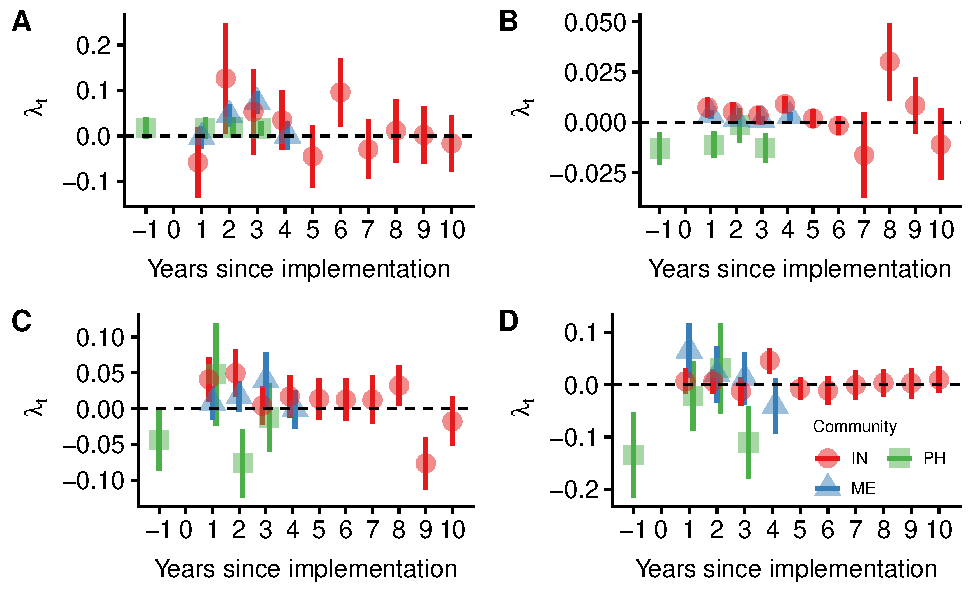
\includegraphics{Villasenor-Derbez_files/figure-latex/unnamed-chunk-8-1.pdf}
\caption{\label{fig:unnamed-chunk-8}\label{fig:indicators}Effect sizes for
marine reserves from Isla Natividad (IN; red cirlcles), Maria Elena (ME;
blue triangles), and Punta Herrero (PH; green squares) for lobster
densities (\emph{Panulirus spp}; A), fish biomass (B), invertebrate
densities (C), and fish densities (D). Plots are ordered by survey type
(left column: invertebrates; right column: fish). Points are jittered
hotizontally to avoid overplotting. Points indicate the effect size and
standard errors. Years have been centered to year of implementation.}
\end{figure}

\begin{figure}
\centering
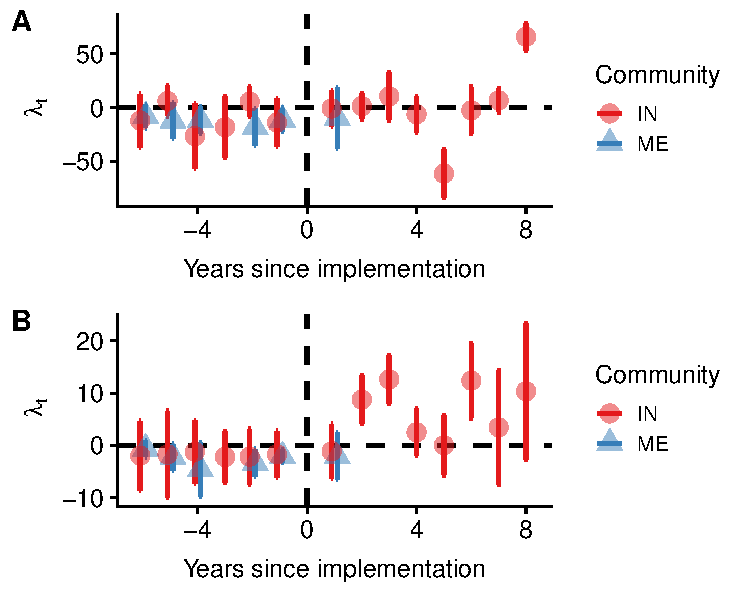
\includegraphics{Villasenor-Derbez_files/figure-latex/unnamed-chunk-9-1.pdf}
\caption{\label{fig:unnamed-chunk-9}\label{fig:lobsters}Effect sizes for
lobster catches (A) and revenues (B) in at Isla Natividad (IN; red
circles) and Maria Elena (ME; blue triangles). Points indicate the
effect size and standard errors. Years have been centered to year of
implementation.}
\end{figure}

\begin{table}[H]

\caption{\label{tab:unnamed-chunk-10}\label{table:indicators}List of indicators used to evaluate the effectiveness of marine reserves, grouped by category.}
\centering
\begin{tabular}[t]{l|l|l}
\hline
Category & Indicator & Units\\
\hline
Biological & Lobster density & org $\mathrm{m}^{-2}$\\
\hline
Biological & Invertebrate density & org $\mathrm{m}^{-2}$\\
\hline
Biological & Fish biomass & Kg $\mathrm{m}^{-2}$\\
\hline
Biological & Fish density & org $\mathrm{m}^{-2}$\\
\hline
Socioeconomic & Income from target species & M MXP\\
\hline
Socioeconomic & Landings from target species & Metric Tonnes\\
\hline
\end{tabular}
\end{table}

\begin{table}[H]

\caption{\label{tab:unnamed-chunk-11}\label{table:ses}Variables for the Social-Ecological System analysis (IN = Isla Natividad, ME = Maria Elena, PH = Punta Herrero). Alphanumeric codes follow \citet{basurto_2013-oq}; an asterisk (*) denotes variables incorporated based on \citet{difranco_2016-Xw} and \citet{edgar_2014-UO}.}
\centering
\resizebox{\linewidth}{!}{\fontsize{11}{13}\selectfont
\begin{tabular}[t]{>{\raggedright\arraybackslash}p{6.5cm}|>{\raggedright\arraybackslash}p{12cm}}
\hline
Variable & Narrative\\
\hline
\multicolumn{2}{l}{\textbf{Resource System (RS)}}\\
\hline
\hspace{1em}RS2 - Clarity of system boundaries: Clarity of geographical boundaries of TURF and reserves & Individual TURF and reserve boundaries are explicitly outlined in official documents that include maps and coordinates. Reserve placement is decided by the community. Fishers use GPS units and landmarks.\\
\hline
RS3 - Size of resource system: TURF Area (Km$^2$) & IN = 889.5; ME = 353.1; PH = 299.7\\
\hline
RS3 - Size of resource system: Reserve area (Evaluated reserve area; Km$^2$) & IN = 2 (1.3); ME = 10.48(0.09); PH = 11.25 (4.37)\\
\hline
\hspace{1em}RS4.1 - Stock status: Status of the main fishery & Lobster stocks are well managed, and are (IN) orhave been (ME, PH) MSC certified.\\
\hline
\hspace{1em}*RS5 - Age of reserves: Years since reserves were implemented & IN = 12; ME = 6; PH = 5\\
\hline
\multicolumn{2}{l}{\textbf{Resource Unit (RU)}}\\
\hline
\hspace{1em}RU5 - Number of units (catch diversity): Number of targeted species & Lobster is their main fishery of these three communities, but they also target finfish. Additionally, fishers from Isla Natividad target other sedentary benthic invertebrates.\\
\hline
\multicolumn{2}{l}{\textbf{Actors (A)}}\\
\hline
\hspace{1em}A1 - Number of relevant actors: Number of fishers & IN = 98; ME = 80; PH = 21\\
\hline
\hspace{1em}*A3 - Isolation: Level of isolation of the fishing grounds & Their fishing grounds and reserves are highly isolated and away from dense urban centers.\\
\hline
\multicolumn{2}{l}{\textbf{Governance system (G)}}\\
\hline
\hspace{1em}GS6.1.4.3 - Territorial use communal rights : Presence of institutions that grant exclusive harvesting rights & Each community has exclusive access to harvest benthic resources, including lobster. These take the form of Territorial User Rights for Fisheries granted by the government to fishing cooperatives.\\
\hline
\hspace{1em}GS6.2 - Operational rules: Rules implemented by individuals atuhorized to partake on collective activities & Fishers have rules in addition to what the legislation mandate. These include larger minimum catch sizes, lower quotas, and assigning fishers to specific fishing grounds within their TURF.\\
\hline
\hspace{1em}GS9.1 - Social monitoring: Monitoring of the activities performed by cooperative members and external fishers & Fishing cooperatives have a group that monitors and enforces formal and internalrules. They ensure fishers of their fishing cooperative adhere to the established rules, and that foreign vessels do not poach their TURF and reserves.\\
\hline
\hspace{1em}GS9.2 - Biophysical monitoring:Monitoring of biological resources, including targeted species & Fishers perform annual standardized underwater surveys in the reserves and fishing grounds. Recently, they have installed oceanographic sensors to monitor oceanographic variables.\\
\hline
GS10.1 - Graduated sanctions & Fishers have penalties for breaking collective-choice rules or fishing inside the reserves. These may range from scoldings and warnings to not being allowed to harvest a particular resource or being expelled from the cooperative.\\
\hline
\end{tabular}}
\end{table}



\end{document}
